\documentclass[compress]{beamer}

\usepackage{thumbpdf}
\usepackage{wasysym}
%\usepackage{ucs}
\usepackage[utf8]{inputenc}
\usepackage[T1]{fontenc}
\usepackage[T2A]{fontenc}
\usepackage{pgf,pgfarrows,pgfnodes,pgfautomata,pgfheaps,pgfshade}
\usepackage{pgfpages}
\usepackage{verbatim}
\usepackage{fancyvrb}
\usepackage{multimedia}
\usepackage{subcaption}
\usepackage{ulem}
\usepackage{textcomp}
\usepackage{tikz}
\usepackage{listings}
\usepackage{amsmath}
\usepackage{amssymb}
\usepackage{graphicx}
%\usepackage{bbding}
\usepackage{multicol}
\usepackage[hyperref=true,backend=biber,sorting=none,backref=true]{biblatex}
\addbibresource{ref.bib}


\makeatletter
\defbeamertemplate*{note page}{mynotes}
{%
  {%
    \scriptsize
    \usebeamerfont{note title}\usebeamercolor[fg]{note title}%
    \ifbeamercolorempty[bg]{note title}{}{%
      \insertvrule{.45\paperheight}{note title.bg}%
      \vskip-.45\paperheight%
      \nointerlineskip%
    }%
    \vbox{
      \hfill\insertslideintonotes{0.45}\hskip-\Gm@rmargin\hskip0pt%
      \vskip-0.45\paperheight%
      \nointerlineskip
      \begin{pgfpicture}{0cm}{0cm}{0cm}{0cm}
        \begin{pgflowlevelscope}{\pgftransformrotate{90}}
          {\pgftransformshift{\pgfpoint{-2cm}{0.2cm}}%
          \pgftext[base,left]{\usebeamerfont{note date}\usebeamercolor[fg]{note date}\the\year-\ifnum\month<10\relax0\fi\the\month-\ifnum\day<10\relax0\fi\the\day}}
        \end{pgflowlevelscope}
      \end{pgfpicture}}
    \nointerlineskip
    \vbox to .45\paperheight{\vskip0.5em
      \hbox{\insertshorttitle[width=8cm]}%
      \setbox\beamer@tempbox=\hbox{\insertsection}%
      \hbox{\ifdim\wd\beamer@tempbox>1pt{\hskip4pt\raise3pt\hbox{\vrule
            width0.4pt height7pt\vrule width 9pt
            height0.4pt}}\hskip1pt\hbox{\begin{minipage}[t]{7.5cm}\def\breakhere{}\insertsection\end{minipage}}\fi%
      }%
      \setbox\beamer@tempbox=\hbox{\insertsubsection}%
      \hbox{\ifdim\wd\beamer@tempbox>1pt{\hskip17.4pt\raise3pt\hbox{\vrule
            width0.4pt height7pt\vrule width 9pt
            height0.4pt}}\hskip1pt\hbox{\begin{minipage}[t]{7.5cm}\def\breakhere{}\insertsubsection\end{minipage}}\fi%
      }%
      \setbox\beamer@tempbox=\hbox{\insertshortframetitle}%
      \hbox{\ifdim\wd\beamer@tempbox>1pt{\hskip30.8pt\raise3pt\hbox{\vrule
            width0.4pt height7pt\vrule width 9pt
            height0.4pt}}\hskip1pt\hbox{\insertshortframetitle[width=7cm]}\fi%
      }%
      \vfil}%
  }%
  \ifbeamercolorempty[bg]{note page}{}{%
    \nointerlineskip%
    \insertvrule{.55\paperheight}{note page.bg}%
    \vskip-.55\paperheight%
  }%
  \vskip.25em
  \nointerlineskip
  \insertnote
}
\makeatother

\setbeameroption{show notes}
\setbeamertemplate{note page}[mynotes]

% Do you want the notes to end up in the PDF?
% \setbeameroption{show notes on second screen=right}
\setbeameroption{hide notes}

\usepackage{epigraph}
\setlength{\epigraphwidth}{.8\textwidth}

\usepackage{DejaVuSansMono}

% Adjust the colours to fit your design
\definecolor{mainthemecolour}{rgb}{0.42,0.48,0.37}
\definecolor{mainthemecolourlight}{rgb}{0.63,0.72,0.57}
\definecolor{mainthemecolourstrong}{rgb}{0.40,0.68,0.18}
\definecolor{mid-gray}{gray}{0.7}

\definecolor{greenstrong}{rgb}{0.58,0.77,0.29}
\definecolor{redstrong}{rgb}{0.81,0.22,0.23}
\definecolor{fglisting}{gray}{0.3}
\definecolor{bglisting}{gray}{1}
\definecolor{fgshell}{gray}{1}
\definecolor{bgshell}{gray}{0.1}
\definecolor{bgshelllight}{gray}{0.8}


% Some in-code macros - a bit buggy, but useful
\newcommand{\hl}[1]{\textcolor{greenstrong}{\texttt{#1}}}
\newcommand{\hlErr}[1]{\textcolor{redstrong}{\texttt{#1}}}
\newcommand{\hlOk}[1]{\textcolor{green}{\texttt{#1}}}
\newcommand{\hlInv}[1]{\colorbox{bgshell}{\textcolor{fgshell}{\texttt{#1}}}}

\newcommand{\unhl}[1]{\textcolor{gray}{#1}}
\newcommand{\clda}[0]{$\textcolor{blue}{\lambda}$}
\newcommand{\carr}[0]{$\textcolor{purple}{\rightarrow}$}
\newcommand{\cbind}[0]{\textbf{\texttt{$>\!\!>\!\!=$}}}
\newcommand{\codedots}[0]{\textcolor{mid-gray}{...}}

\usetheme{elegance}

\lstnewenvironment{cxxcode}
    {\lstset
        { escapeinside={@}{@}
        , gobble=8
        , showstringspaces=false
        , basicstyle=\color{fglisting}
        , rulecolor=\color{mainthemecolourlight}
        }
    }
    {}

\lstnewenvironment{cxxcodebox}
    {\lstset
        { escapeinside={@}{@}
        , gobble=6
        , showstringspaces=false
        , basicstyle=\color{fglisting}
        , frame=lr
        , rulecolor=\color{mainthemecolourlight}
        }
    }
    {}

\lstnewenvironment{shellcode}
    {\lstset
        { escapeinside={@}{@}
        , gobble=7
        , showstringspaces=false
        , basicstyle=\color{fgshell}
        , backgroundcolor=\color{bgshell}
        }
    }
    {}


% Marking points to use in Tikz
\usetikzlibrary{arrows,shapes}
\newcommand{\tikzmark}[1]{\tikz[remember picture] \node[coordinate] (#1) {#1};}

% Fragile frames
\newenvironment{xframe}[1][]
  {\begin{frame}[fragile,environment=xframe,#1]}
  {\end{frame}}



\title{Elegance}
\subtitle{An elegant theme for Beamer}
\author{Ivan Čukić}

\institute{\color{white}
    email@address.org \\
    http://address.org
} %
\date{\footnotesize\color{mainthemecolour} Conference, City 2016. }




\begin{document}

\maketitle

\section{Introduction}
	\subsection{part1.1}
		\begin{xframe}{Backgound}
			Turbulent combustion is encountered in most practical combustion system such as rocket, ICE, and aircraft engien.
			\begin{figure}
				\begin{minipage}{3.5cm}
					\centering
					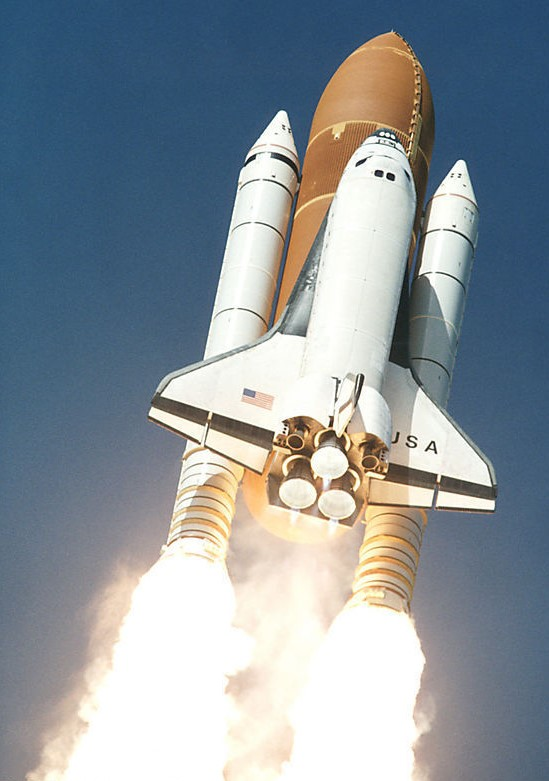
\includegraphics[height=3.5cm, width=3cm]{../pic/rocket.jpg}
				\end{minipage}%
				\begin{minipage}{7.5cm}
					\centering
					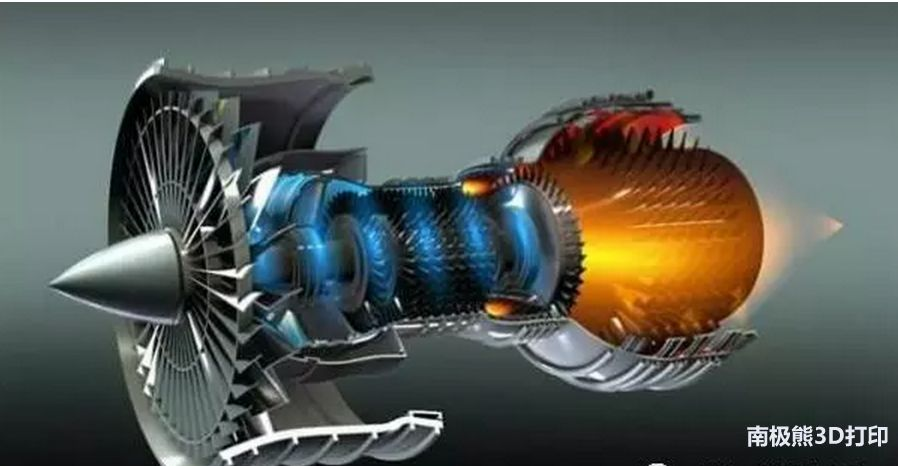
\includegraphics[height=3.5cm, width=7cm]{../pic/engien.jpg}
				\end{minipage}%
			\end{figure}
			\pause
			Meaningful to practical systems:
			\begin{enumerate}[(a)]
				\item 
				Improve efficiency, meet demanding standards\cite{RN1}.
				\item
				Reduce pollution, environment friendly.
			\end{enumerate}
		\end{xframe}
	\subsection{part1.3}
		\begin{xframe}{Numerical simulation of flowfield}
			Based on CFD, there're 3 possible approaches:
			\begin{enumerate}[(a)]
				\item{Direct Numerical Simulation(DNS)}\newline
					--Precise, but costly(Tremendous memory and CPU). %\XSolid
				\item Large Eddy Simulation(LES)\newline
					--Compromise between accuracy and computational cost. %\Checkmark
				\item Reynolds Averaged Navier-Stokes(RANS)\newline
					--Inaccurate for combustion phenomenon. %\XSolid
			\end{enumerate}
			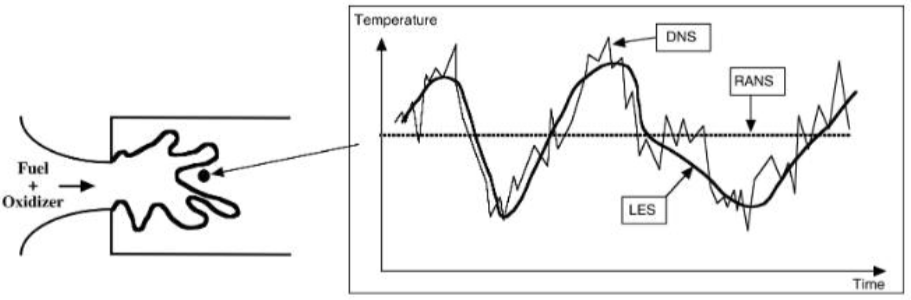
\includegraphics[width=11cm, height=3cm]{../pic/comparision.png}
		\end{xframe}
	\subsection{part1.4}
		\begin{xframe}{Numerical simulation of flame}
			Although based on LES, traditional flame models are inadequate:
			\begin{itemize}
				\item
					Distribution of flame properties are mannually assumed.
				\item
					Parameter tuning may be unphysical.
			\end{itemize}
			\pause
			These drawbacks are overcame by the turbulent flamelet model to be introduced:
			\begin{itemize}
				\item
					Designed especially for LES, with fewer approximation.
				\item
					Relations are provided through scaling law, which is based on DNS database\cite{RN2}.
			\end{itemize}		
		\end{xframe}
\section{Turbulent Flamelet Model}
	\subsection{part2.1}
		\begin{xframe}{Theory}
			Original G.E. in the context of LES:
			\begin{equation}
				\frac{\partial \bar{\rho}\tilde{Z}}{\partial t} + \nabla \cdot (\bar{\rho} \tilde{Z}\tilde{\vec{u}}) = \nabla \cdot [\bar{\rho}(D+D_T)\nabla\tilde{Z}]
			\end{equation}
			\begin{equation}
				\frac{\partial \bar{\rho}\tilde{Y_i}}{\partial t} + \nabla \cdot (\bar{\rho} \tilde{Y_i}\tilde{\vec{u}}) = \nabla \cdot [\bar{\rho}(D+D_T)\nabla\tilde{Y_i}] + \overline{\omega_i}
			\end{equation}
			\pause
			After coordinate transformation$(x_1,x_2,x_3,t)\rightarrow(Z,Z_2,Z_3,\tau)$:
			\begin{equation}
				\begin{split}
					\bar{\rho}\frac{\partial \tilde{Y_i}}{\partial \tau} + \bar{\rho} \Big(\tilde{\vec{u}} \cdot \nabla_\perp \tilde{Y_i} + \frac{\partial \tilde{Y_i}}{\partial Z_2}\frac{\partial Z_2}{\partial t} + \frac{\partial \tilde{Y_i}}{\partial Z_3}\frac{\partial Z_3}{\partial t}\Big) = \frac{\bar{\rho}\chi}{2Le_T}\frac{\partial^2 \tilde{Y_i}}{\partial^2 \tilde{Z}}\\ + \frac{\partial \tilde{Y_i}}{\partial \tilde{Z}}\nabla\cdot\Bigg[\bar{\rho}(\mathcal{D}_{T,i}-\mathcal{D}_T)\vec{n}\cdot\frac{\partial \tilde{Z}}{\partial \vec{n}}\Bigg] + \nabla \cdot (\bar{\rho}\mathcal{D}_{T,i}\nabla_\perp\tilde{Y_i}) + \overline{\omega_i}
				\end{split}	
			\end{equation}
		\end{xframe}
	\subsection{part2.2}
		\begin{xframe}{Laminar Flamelet assumption}
			Locally, the characteristic timescale of chemical reaction is much smaller that that of flow$(t_c \ll t_f)$.\newline
			Thus, local flame structure can be described by the difffusion flame under counterflow configuration.
			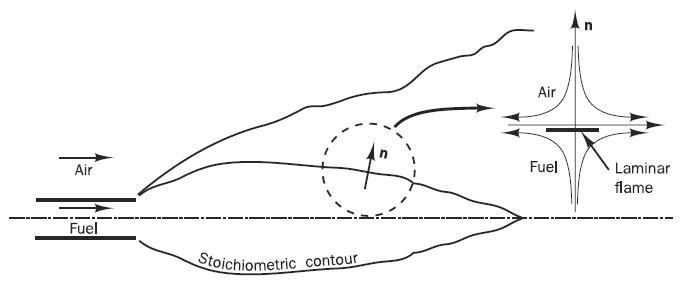
\includegraphics[width=10cm, height=3cm]{../pic/flamelet.png}
			
			Each micro flamelet can be described by $Z$ and $\chi$:
			\begin{itemize}
				\item $Z$ describes chemical reaction.
				\item $\chi$ indicates turbulence stretching effect.
			\end{itemize}
			Thus, a database can be pre-computed for later looking-up. 
		\end{xframe}
	\subsection{part2.3}
		\begin{xframe}{Turbulent Flamelet}
			\begin{multicols}{2}
				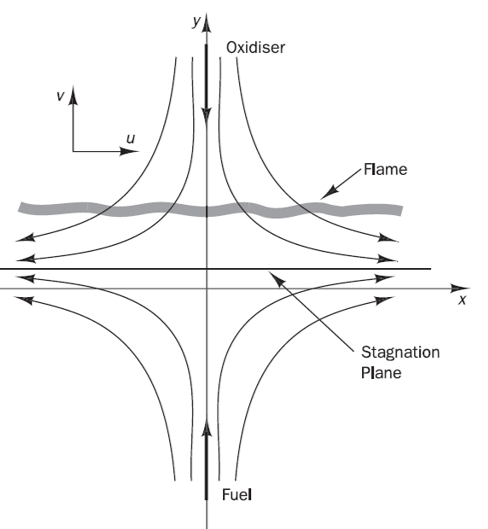
\includegraphics[width=5.5cm, height=7cm]{../pic/counterflow.png}	
				
				Unlike the laminar flamelet introduced above,\\
				G.E. of the counterflow flame is slightly modified by our turbulet flamelet model from
				\begin{equation}
					\rho \frac{D Y_i}{D t} = \mathcal{D}_i\frac{\partial^2 Y_i}{\partial^2 x} + \omega_i(T, \vec{Y})
				\end{equation}
				to
				\begin{equation}
					\bar{\rho} \frac{D \tilde{Y_i}}{D t} = \mathcal{D}_i\frac{\partial^2 \tilde{Y_i}}{\partial^2 x} + \tilde{\omega_i}(\tilde{T}, \tilde{\vec{Y}})
				\end{equation}
				The two equations share similar form, but have totally different meanings.
			\end{multicols}
		\end{xframe}
	\subsection{part2.4}
		\begin{xframe}{Solution procedure}
			Based on the filtered turbulent flamelet database generated in the way descirbed above, the full solution procedure that incorporates a CFD solver can be described as follows:
			\centering
			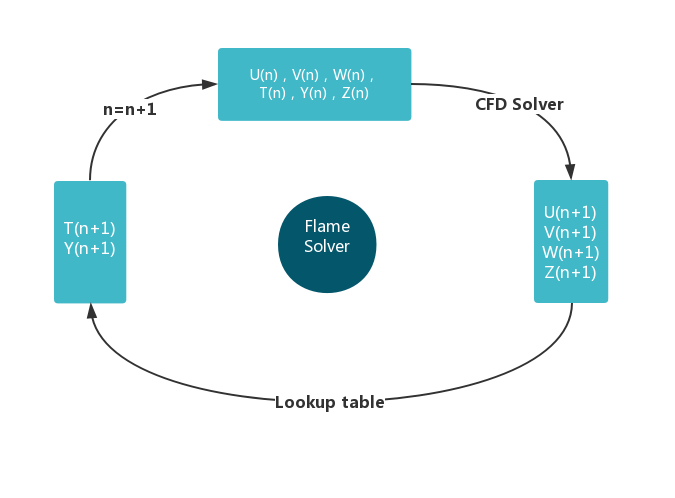
\includegraphics[width=9cm, height=6.5cm]{../pic/solver.png}
		\end{xframe}
\section{Numerical Results}
	\subsection{part3.1}
		\begin{xframe}{Comparsion of ``S'' curve}
			The $T_{max}$ plot:
			\begin{itemize}
				\item
					One of the most convincing testing cases.
				\item
					Difference and transition position are clearly revealed\cite{RN11}.
			\end{itemize}			
			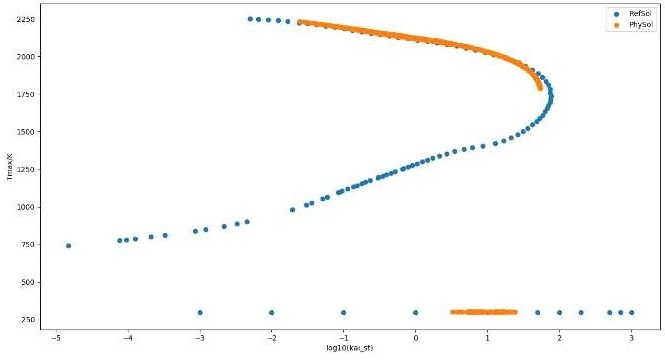
\includegraphics[width=11cm, height=6cm]{../pic/Tmax.jpg}	
		\end{xframe}
	\subsection{part3.2}
		\begin{xframe}{Standard case}
			Comparsion between experimental data, which is widely used as benchmark\cite{RN14}.
			\begin{figure}
				\begin{minipage}{3.5cm}
					\centering
					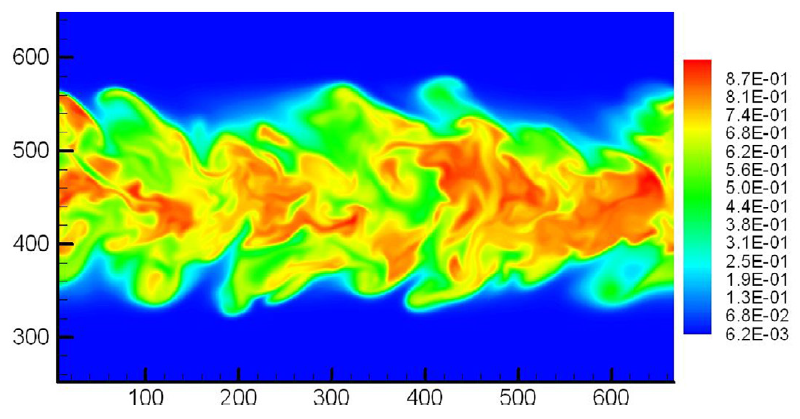
\includegraphics[height=3cm, width=5cm]{../pic/slice.png}
				\end{minipage}%
				\begin{minipage}{7.5cm}
					\centering
					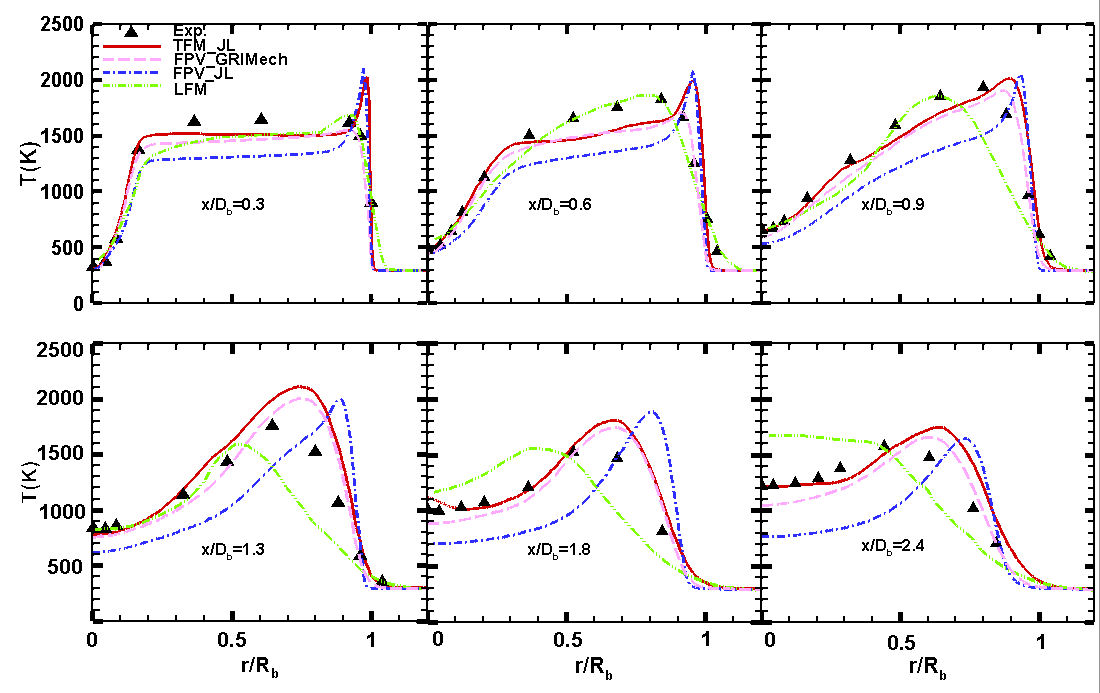
\includegraphics[height=5.5cm, width=7cm]{../pic/line.png}
				\end{minipage}%
			\end{figure}
		\end{xframe}
\section{Conclusions}
	\subsection{part4.1}
		\begin{xframe}{Conclusions}
			\begin{itemize}
				\item
					Turbulent flamelet model has good agreement with experimental data.
				\pause
				\item
					Numerical simulation based on Large Eddy Simulation(LES) shows better resolution of flame structures.
				\pause
				\item
					Flamelet modeling based on the filtered G.E. is physically effective for combustion problem.
			\end{itemize}	
		\end{xframe}
	\subsection{part4.2}
		\begin{xframe}{Reference}
			\printbibliography
		\end{xframe}
\end{document}
